\section{生成阀盖三视图}
\begin{procedure}
\item 打开“调压阀阀盖立体图.dwg”文件,并另存为“调压阀阀盖布局图.dwg”。

这样做的目的是为了保护源文件,以防止误操作后可进行有效的恢复之前的工作。AutoCAD本身并没有要求这样做。
\item 新建布局。

新建布局的方法有:
\begin{itemize}
\item 键盘输入LAYEROUT命令中的【新建N】选项。
\item 点击【插入】菜单中【布局】子菜单中的【新建布局】项。
\item 点击【插入】菜单中【布局】子菜单中的【创建布局向导】项。
\item 右击【模型】和【布局】
\includegraphics[scale=0.8]{buju.png} 区域,在弹出菜单中选择【新建布局】项。
\item 单击【模型】和【布局】
\includegraphics[scale=0.8]{buju.png} 区域中的【布局1】或【布局2】选项卡。
\item 点击【布局】工具栏中的【新建布局图标】
\includegraphics[scale=0.7]{buju1.png}
\end{itemize}
在此我们以【创建布向导】的方式来讲述如何新建布局。启动【创建布局】向导后会弹出图\ref{fig:bujuxiangdao1}所示对话框。
\begin{figure}[htbp]
\centering
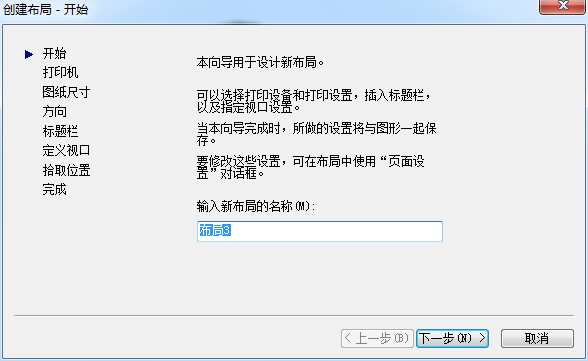
\includegraphics[scale=0.8]{bujuxiangdao1.png}
\caption{创建布局-开始对话框}\label{fig:bujuxiangdao1}
\end{figure}

此时,输入布局的名称并单下一步,弹出图\ref{fig:bujuxiangdao2}所示打印机设置对话框,将打印机设置为“DWG TO PDF.pc3"。实际工作中则就设置为可用的打印设备。
\begin{figure}[htbp]
\centering
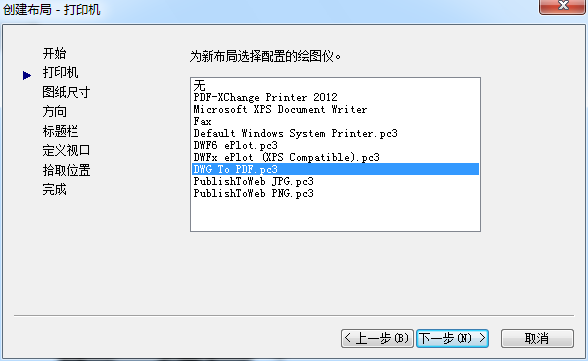
\includegraphics[scale=0.7]{bujuxiangdao2.png}
\caption{创建布局-打印机}\label{fig:bujuxiangdao2}
\end{figure}

设置完打印机后,单击下一步,弹出图\ref{fig:bujuxiangdao3}所示的图纸尺寸设置对话框。单击下拉框,将图纸设置为“ISO A4(297.00x210.00毫米)”,图形单位设置为毫米。
\begin{figure}[htbp]
\centering
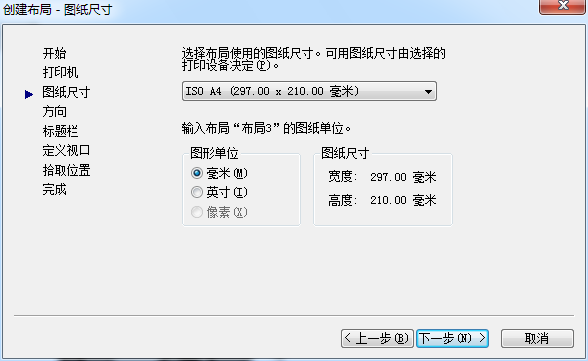
\includegraphics[scale=0.7]{bujuxiangdao3.png}
\caption{创建布局-图纸尺寸}\label{fig:bujuxiangdao3}
\end{figure}

设置完成后,单击下一步,弹出图\ref{fig:bujuxiangdao4}所示的方向设置对话框。此时将图形在图纸上的方向设置为横向。
\newpage
\begin{figure}[htbp]
\centering
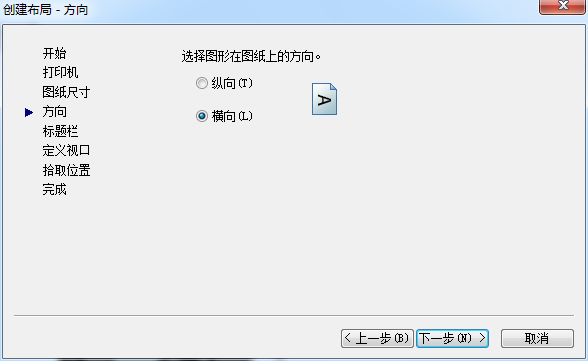
\includegraphics[scale=0.7]{bujuxiangdao4.png}
\caption{创建布局-方向}\label{fig:bujuxiangdao4}
\end{figure}

设置完成后,单击下一步,弹出图\ref{fig:bujuxiangdao5}所示的标题栏设置对话框。此时,将标题栏路径设置为无。
\begin{figure}[htbp]
\centering
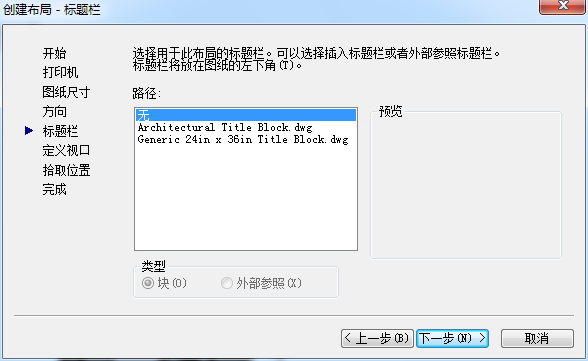
\includegraphics[scale=0.7]{bujuxiangdao5.png}
\caption{创建布局-标题栏}\label{fig:bujuxiangdao5}
\end{figure}

设置完成后,单击下一步,弹出图\ref{fig:bujuxiangdao6}所示的定义视口对话框。视口设置中单个表示创建一个视口,标准三维工程视图创建四个相等三个视口,阵列用于创建指定行和列的视口中。视口比例用于设置视口中显示对象的比例。由于生成三视图不需要用视口,因此在视口设置中选择无。
\newpage
\begin{figure}[htbp]
\centering
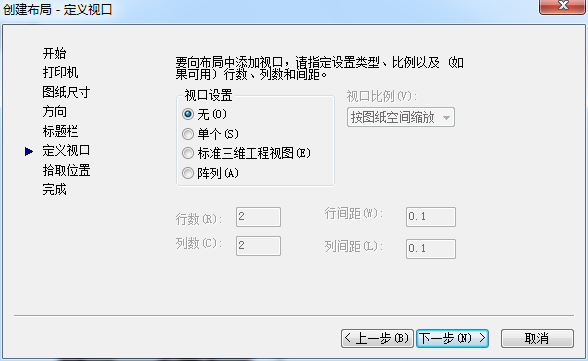
\includegraphics[scale=0.7]{bujuxiangdao6.png}
\caption{创建布局-定义视口}\label{fig:bujuxiangdao6}
\end{figure}

设置完成后,单击下一步,并点击完成,结束布局创建。
\item 从布局空间切换至模型空间。
\item 将工作空间由AutoCAD经典切换为三维建模,如图\ref{fig:sanweijianmo}所示。
\begin{figure}[htbp]
\centering
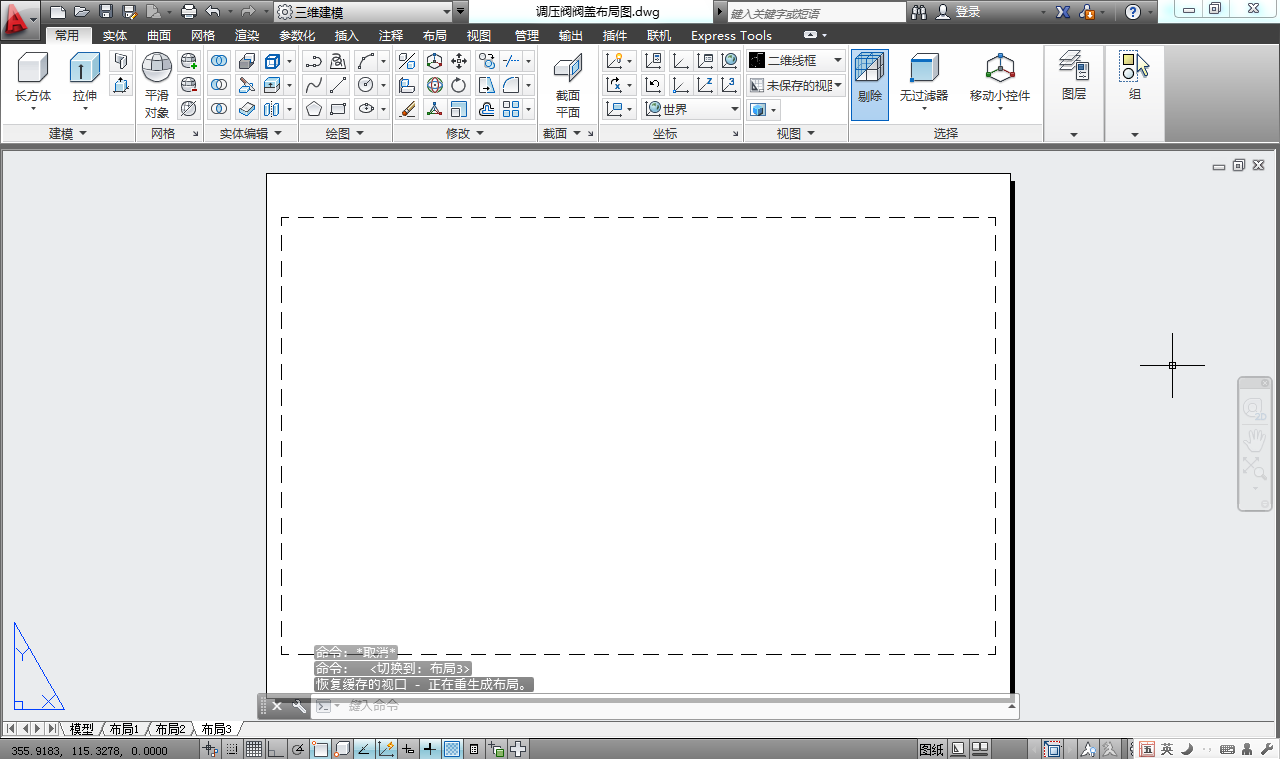
\includegraphics[scale=0.3]{sanweijianmo.png}
\caption{创建布局-定义视口}\label{fig:sanweijianmo}
\end{figure}
\item 创建基础视图。
启动创建基础视图的方法有:
\begin{itemize}
\item 键盘输出VIEWBASE。
\item 点【布局选项卡】中的【基础】图标
\includegraphics[scale=0.5]{viewbase.png},从下拉框中的选择
\includegraphics[scale=0.45]{comefrommodel.png}项
\end{itemize}
\newpage
启动命令后,选择从模式空间生成。
\begin{lstlisting}
|命令: VIEWBASE|
|指定模型源 [模型空间(M)/文件(F)] $<$模型空间$>$:
\end{lstlisting}
从模型空间中选择阀盖实体。
\begin{lstlisting}
|选择对象或 [整个模型(E)] $<$整个模型$>$: 找到 1 个|
|选择对象或 [整个模型(E)] $<$整个模型$>$:|
\end{lstlisting}
选择新创建的布局3作为生成的图纸。
\begin{lstlisting}
|输入要置为当前的新的或现有布局名称或 [?] $<$布局3$>$:|
|恢复缓存的视口 - 正在重生成布局。|
|命令:|
|类型 = 基础和投影  隐藏线 = 可见线和隐藏线  比例 = 1:1|
\end{lstlisting}
指定主视图的位置,如图\ref{fig:fagaibaseview1}所示。
\begin{lstlisting}
|指定基础视图的位置或 [类型(T)/选择(E)/方向(O)/隐藏线(H)/|
|比例(S)/可见性(V)] $<$类型$>$:|
|选择选项 [选择(E)/方向(O)/隐藏线(H)/比例(S)/可见性(V)/移动(M)|
|/退出(X)] $<$退出$>$:|
\end{lstlisting}
\begin{figure}[htbp]
\centering
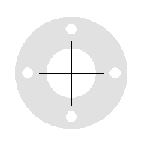
\includegraphics[scale=1.4]{fagaibaseview1.png}
\caption{指定主视图位置}\label{fig:fagaibaseview1}
\end{figure}
选择左视图的投影视图位置
\begin{lstlisting}
|指定投影视图的位置或 $<$退出$>$:|
\end{lstlisting}
\begin{figure}[htbp]
\centering
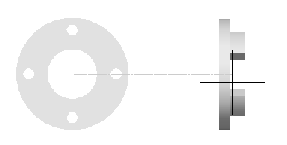
\includegraphics[scale=1.4]{fagaibaseview2.png}
\caption{指定左视图位置}\label{fig:fagaibaseview2}
\end{figure}
\newpage
选择俯视图的投影视图位置
\begin{lstlisting}
|指定投影视图的位置或 [放弃(U)/退出(X)] $<$退出$>$:|
|指定投影视图的位置或 [放弃(U)/退出(X)] $<$退出$>$:|
\end{lstlisting}
\begin{figure}[htbp]
\centering
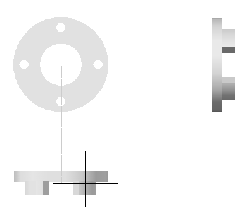
\includegraphics[scale=1.2]{fagaibaseview3.png}
\caption{指定左视图位置}\label{fig:fagaibaseview3}
\end{figure}
最终结果如图\ref{fig:fagaibaseview4} 所示。
\begin{figure}[htbp]
\centering
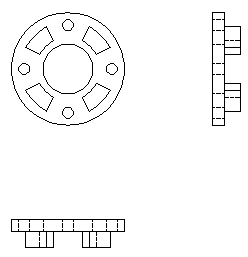
\includegraphics[scale=1.2]{fagaibaseview4.png}
\caption{阀盖三视图}\label{fig:fagaibaseview4}
\end{figure}
\end{procedure}
\endinput